% !TEX root = ../../Thesis_main.tex
\section{Context}
\subsection{Problem of 3D reconstruction}

Problem of 3D reconstruction can be described as following: given some 2D/2.5D data from sensors (e.g. photos, videos, images from depth sensors, LiDAR data, in rare cases acoustic or radar images), create a model of the invironment in which this data was recorded such that projections to perspectives from which it was registered will give the same images. This problem arises in many different fields from biomediciny to astronomy, but in this work a scope is reduced to human scale indoor environments in modern countries.

\begin{figure}
	\centering
    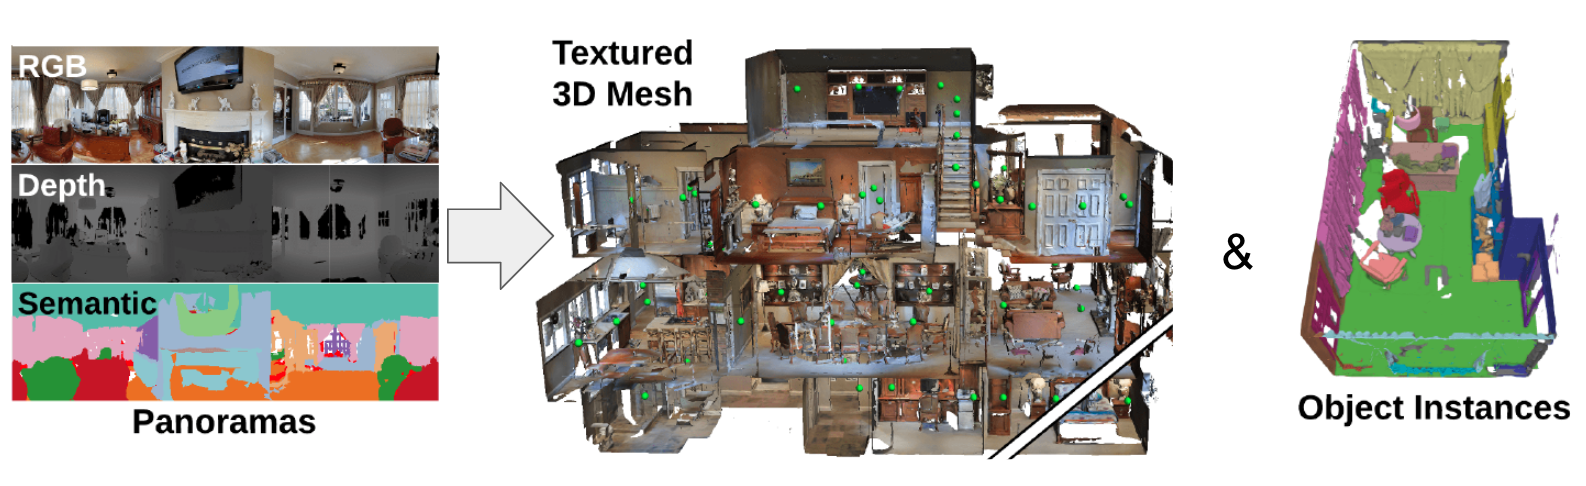
\includegraphics[width=\textwidth]{Figures/reconstruction_steps.png}
    \caption{Using sensory data (RGB-D) reconstruct 3D model of environments with shapes and locations of objects. In some problem formulations also with textures and reflective radiance functions, camera parameters and lighting conditions.}
    \label{fig:reconstruction_steps}
\end{figure}


\subsection{Approaches for solving 3D Reconstruction problem}

Solutions for a reconstruction problem can be grouped in two major groups: 1) Geometric approach - when problem is represented as optimisation of scene state given constrains on projections of scene state to data, 2) Machine Learning approach - inverse model is optimisation.

If $X$ - is scene data, $z$ - is the state of the scene, and $g_i(z)$ - projection function of 3D scene $z$ state to perspective $i$, then to find an optimal 3D reconstruction, one solves this minimisation problem:
\begin{equation}
z_{rec} = \min_z\sum_i|X_i-g_i(z)|_2 .
\end{equation}

This approach only solves problem for once scene and does not provide any semantic information about it, only basic geometric information. 
The second approach is more modern and better fitted for machine learning applications, because instead of optimizing state of the scene, it's optimizes a model that performs computation from input data to some semantic (intrinsic) parameters, and can be described as following optimisation procedure:
\begin{equation}
\min_\theta\sum_i|X_i-g_i(f_\theta(\pi))|_2,\ \ \pi=I_\theta(\{X_i\}_i),\ \ z=f_\theta(\pi),
\end{equation}
where $\pi$ - are scene parameters, $f_\theta(\pi)$ - is a generative model that generates 3D state $z$ and it's function is determined by tunable parameters $\theta$.

In reconstruction process information can be introduced in two possible ways: 1) input signal - data measured by some spatial sensor, 2) by adding a priori knowledge while training the Inverse model or by design choice of reconstruction algprithm. Between the two source exist a fundamental trade-off and detirmination of which is dominant can be quite difficult \cite{tatarchenko2019single}.

\subsection{3D data representations}

We can describe a 3D object in multiple ways, and codification of it's properties has ramifications about capturing different information about objects and scenes, as well as kinds of models that can regenerate them or computational resources needed to process it.
Each representation has it's own pros and cons. We assume 3D information representation to be positive effective and usefull if it captures more relevant information with less storage requirement (compression), increases signal to noise ratio of data, captures shape and texture properties with minimum trade-off.

Using neural network to estimate 3D properties really depends on shape representation space, here are some popular examples of 3D data representations:
\begin{enumerate}
	\item \textbf{Multiple 2D projections} - captures surface texture, highly redundant representation if images overlap, also vulnerable to optic illusions.
	\item \textbf{3D Voxel grid} - simple, most of the time can be sparse, represents rough volumetric properties vell but losses most of surface properties, can be generated by deconvolutional network in hour-glass, auto-encoder or GAN architectures.
	\item \textbf{RGB-D (2.5D)} images are widespread because of cheap measurement devices, capture volumentric depth but succeptable to occlusion of bodies in a scene and records a lot of noise with actual signal.
	\item \textbf{Point Cloud} - are sparse in a sense that they don't capture empty space, losing all surface properties besides color and estimated normals and most of volumetric properties, sometimes can be combined with previous item.
	\item \textbf{Surface mesh} - not generated exactly but reconstructed from one of previous items, might be possible to generate with geometric deep learning methods.
	\item \textbf{Signed Distance Field functions (SDF)} - representation of shape as an implicit function with it's kernel representing body's surface.
\end{enumerate}

Multiple view projections shown to be a great way in discriminative tasks like in MVCNN paper~\cite{su15mvcnn}, but in a last year multiple papers used multiple-view projections in a generative setting, here are several examples~\cite{Soltani_2017_CVPR,girdhar2016learning,lin2017learning,Ulusoy_2017_CVPR,tatarchenko2016multi}.

In work by Soltani~\cite{Soltani_2017_CVPR} combination 2D and 2.5D projections is used in a auto-encoder style architecture to capture distribution of shapes of objects from ShapeNet dataset~\cite{chang2015shapenet}.

In Paper by Chen-Hsuan Lin~\cite{lin2017learning} two step network first tries to encode image to latent code, then create multiple projections of multiple points from this code from different angles then combining those points in to 3D point cloud regularizing shape and re-projecting with pseudo-renderer to estimate loss function.

Similar but yet different approaches is used in work supervised by Abhinav Gupta~\cite{girdhar2016learning} where projections used to train in auto-encoder architecture latent representation of 3D shapes and 2D sub-network is connected to latent representation and used in inference time.

Series of papers are using Point clouds to capture volumetric properties of shapes, like PointNet papers~\cite{qi2016pointnet,qi2017pointnet++}. They show good performance on volumetric benchmarks but don't provide any way to work with surfaces of objects without using some other surface reconstruction method first.